\documentclass[aps,prd,onecolumn,superscriptaddress,nofootinbib]{revtex4-2}

% Packages
\usepackage[utf8]{inputenc}
\usepackage[T1]{fontenc}
\usepackage{lmodern}
\usepackage{amsmath,amssymb,bm,mathtools,amsthm}
\usepackage{graphicx}
\usepackage{adjustbox}
\usepackage{xcolor}
\usepackage{microtype}
\usepackage[unicode, pdfencoding=auto, psdextra]{hyperref}
\usepackage{enumitem}
\usepackage{tikz}
\usetikzlibrary{arrows.meta,positioning,fit,calc,shapes.geometric,shapes.multipart,backgrounds}

% Colors for flowchart
\definecolor{flowBlue}{HTML}{1F77B4}
\definecolor{flowPurple}{HTML}{9467BD}
\definecolor{flowGreen}{HTML}{2CA02C}
\definecolor{flowOrange}{HTML}{FF7F0E}
\definecolor{flowRed}{HTML}{D62728}

% Hyperref
\hypersetup{
  colorlinks=true,
  linkcolor=blue,
  citecolor=blue,
  urlcolor=blue
}

% PDF string sanitization
\pdfstringdefDisableCommands{%
  \def\OmL{OmegaLambda}%
  \def\Omm{Omega m0}%
  \def\cgeo{cgeo}%
  \def\alphaM{alphaM}%
  \def\eps{epsilon}%
  \def\boxed#1{#1}%
  \def\mu{mu}%
  \def\alpha{alpha}%
  \def\alpha_M{alphaM}%
  \def\Omega_\Lambda{OmegaLambda}%
}

% Math tweaks
\allowdisplaybreaks

% Macros
\providecommand{\mpl}{M_{\rm P}}
\providecommand{\OmL}{\Omega_\Lambda}
\providecommand{\Omm}{\Omega_{m0}}
\providecommand{\cgeo}{c_{\rm geo}}
\providecommand{\alphaM}{\alpha_M}
\providecommand{\eps}{\varepsilon}

% Theorem-like environments
\newtheorem{definition}{Definition}
\newtheorem{hypothesis}{Hypothesis}
\newtheorem{lemma}{Lemma}
\newtheorem{proposition}{Proposition}
\newtheorem{theorem}{Theorem}
\newtheorem{corollary}{Corollary}

\begin{document}

\title{State-Dependent Gravity from Modular Information:\\
A KMS/FDT Linear-Response Framework (Conditional)}

\author{[Authors]}
\affiliation{[Institutions]}
\date{}

\begin{abstract}
We present a \emph{conditional} information-theoretic framework in which finite local information capacity produces a \emph{state-dependent} gravitational response. The key working assumption is replaced by a \textbf{KMS-normalized linear-response (A2–KMS) hypothesis}: in the small-wedge, MI/moment-kill projector channel, Bisognano–Wichmann (BW) KMS structure and the fluctuation–dissipation theorem (FDT) fix the sign and normalization of the modular susceptibility to $\mathcal O(\ell^4)$, with curvature/contact remainders $\mathcal O(\ell^6)$. We \emph{define} a dimensionless state variable $\eps$ via flat-space modular response, $\delta\!\langle K_{\rm sub}\rangle=(2\pi C_T I_{00})\,\ell^4\,\delta\eps+\mathcal O(\ell^6)$, and \emph{map} $\eps$ to a weak-field coupling through A2–KMS, yielding $\delta G/G=-\beta\,\delta\eps$ with $\beta\equiv 2\pi C_T I_{00}$. A geometric normalization yields a universal weak-field prefactor $5/12=(4/3)\times(5/16)$, implying $\mu(\eps)=1/(1+\tfrac{5}{12}\eps)$ and $a_0=\tfrac{5}{12}\,\OmL^2 cH_0$. The scheme-invariant mapping $\OmL=\beta\,f\,\cgeo\approx 0.685$ (conservative $\pm 5\%$ from shared systematics in $\beta$) preserves EM/GW distances (distance sector kept GR-like).

\emph{New in this version.} We promote A2–KMS to a \textbf{theorem in the Gaussian/Hadamard sector} (free fields, small diamonds, bounded curvature, MI/moment-kill projector): the $\ell^4$ coefficient, FDT positivity, the $5/12$ prefactor, and the $\mathcal O((\ell/L_{\rm curv})^2)$ CHM-vs-half-space KMS defect are established at working order. Beyond free fields, the extension remains a conjectural \emph{proof program}; cosmological applications should be read as \emph{illustrative bounds consistent with} (but not yet proven for) interacting QFTs.
We solve $\eps(a)$ and linear growth $D(a)$ as a KMS/FDT-constrained \emph{fixed point} and report \emph{entropy-constrained variational bounds} on $S_8$ (late-/early-loaded profiles bracket the admissible range), rather than a single fit; our baseline lies within this band. Substrate \emph{structural consistency checks} (HQTFIM and Gaussian chains) confirm algebraic ingredients but are \emph{not} 4D curved-spacetime surrogates. We give explicit falsifiers, conservative uncertainties, and a limitations box (safe-window viability, KMS error, environment gate microphysics, quantum-classical bridge).
\end{abstract}

\maketitle

% ===============================
\section{Scope, Working Order, and Limitations (Read First)}
\label{sec:scope}
\noindent\textbf{Working order.} ``Working order'' means we isolate the isotropic $\ell^4$ contribution in the MI/moment-kill projector channel and treat curvature/contact corrections as $\mathcal O(\ell^6)$.\\[3pt]
\noindent\textbf{Safe window (existence is model dependent).} We assume a nonempty range $\ell$ obeying
\[
\epsilon_{\rm UV}\ll \ell \ll \min\{L_{\rm curv},\lambda_{\rm mfp},m_i^{-1}\}.
\]
In halos with $L_{\rm curv}\sim 10\,\mathrm{Mpc}$, a plausible late-time band is $\ell\in[1,100]\,\mathrm{pc}$; this window can be \emph{absent} in dense regions (star-forming zones, cluster cores).\\[3pt]
\noindent\textbf{KMS applicability (CHM vs.\ half-space).} Exact BW KMS analyticity holds for half-spaces; CHM diamonds approximate it in the safe window. The fractional KMS deviation scales as $\mathcal O((\ell/L_{\rm curv})^2)$ (App.~\ref{app:chm-kms-estimate}).\\[3pt]
\noindent\textbf{State assumption (Hadamard).} We assume locally Hadamard states so that short-distance correlators match Minkowski up to curvature-suppressed terms. If data reveal departures from Hadamard short-distance structure in the projector channel, the framework is \emph{falsified}.\\[3pt]
\noindent\textbf{Proven vs.\ conjectural.} \emph{Proven (Gaussian/Hadamard sector at working order):} $\ell^4$ modular coefficient equals the flat-space value; FDT positivity in the projected channel; $5/12$ weak-field prefactor; CHM KMS defect $\sim \mathcal O((\ell/L_{\rm curv})^2)$. \emph{Conjectural (program for general fields):} control of KMS kernel beyond free fields, full curved-diamond relative-entropy/canonical-energy equivalence, and uniqueness of the coupling to $M^2$.\\[3pt]
\noindent\textbf{Distances kept GR-like.} We enforce $\alphaM\simeq 0$ in the distance sector; null geometry and EM/GW distances are unmodified at working order.\\[3pt]
\noindent\textbf{Environment gate is illustrative.} The gate $F_g(g/a_0)$ is a minimal compliance envelope: $F_g\!\to\!0$ in strong fields (Solar System), $F_g\!\to\!1$ in weak fields; a microscopic derivation is future work.\\[3pt]
\noindent\textbf{Substrate tests are algebraic checks.} HQTFIM/Gaussian runs test the algebraic structure (first-law channel, constant+log trend, plateau, FDT-positivity). They are \emph{not} physical surrogates for 4D curved spacetime.\\[3pt]
\noindent\textbf{Falsifiers and uncertainties.} We list sharp falsifiers (Sec.~\ref{sec:falsifiers}) and adopt a conservative $\pm 5\%$ uncertainty on $\beta$ (shared systematics), with angle-invariance presented as a \emph{null} residual test rather than a precision claim.

% ===============================
\section{A2–KMS Hypothesis (Definition, Channel, and Positivity)}
\label{sec:A2KMS}
\paragraph{BW recap.} The Minkowski vacuum restricted to a Rindler half-space is a KMS state at inverse temperature $\beta_{\rm KMS}=2\pi/\kappa$ with respect to boost flow (Bisognano–Wichmann).\\[3pt]
\noindent\textbf{A2–KMS (boxed).}
\begin{hypothesis}[A2–KMS (working order)]
\label{hyp:A2KMS}
In the MI/moment-kill projector channel for small CHM diamonds in a safe window, the wedge state inherits BW KMS analyticity up to $\mathcal O((\ell/L_{\rm curv})^2)$. The linear-response susceptibility relating modular perturbations to boost-energy flux is fixed by the KMS two-point function, is positive (FDT), and its finite $\ell^4$ coefficient equals the flat-space value at working order:
\[
\delta\langle K_{\rm sub}\rangle=(2\pi C_T I_{00})\,\ell^4\,\delta\eps+\mathcal O(\ell^6),\qquad
\frac{\delta G}{G}=-\beta\,\delta\eps,\ \ \beta\equiv 2\pi C_T I_{00}.
\]
\end{hypothesis}
\noindent\textbf{Boxed reminder (constitutive \& falsifiable).} \emph{Equation $\delta G/G=-\beta\,\delta\varepsilon$ is a \textbf{constitutive closure at working order} in the BW/KMS projector channel. It is \textbf{not} a macroscopic thermodynamic law and is \textbf{falsified} by any of: persistent $\ell^4\log\ell$ residuals in the MI/moment-kill channel, violation of the EM/GW distance bound, or an $\Omega_\Lambda$ inconsistent with $\beta f c_{\rm geo}$.}
\noindent\emph{Remarks.} (i) Exact KMS is half-space; diamond validity is approximate and quantified in App.~\ref{app:chm-kms-estimate}. (ii) FDT positivity enforces $\Delta S\ge 0$ in this channel without invoking macroscopic heat. (iii) ``Temperature'' is the KMS normalization for boost flow, not a literal bath. (iv) \textbf{State class:} we assume locally Hadamard states so that the short-distance two-point structure is Minkowski-like; large deviations would invalidate the working-order reduction and thus \emph{falsify} the framework.

\subsection*{Theorem (Gaussian/Hadamard A2–KMS; working order)}
\label{sec:theorem}
\begin{theorem}[Free fields, Hadamard states, small diamonds]
Let $\mathcal Q$ be a free (Gaussian) QFT on a globally hyperbolic spacetime and $\rho$ a locally Hadamard state. For a causal diamond of radius $\ell$ satisfying $\ell\ll L_{\rm curv}$, the MI/moment-kill projector isolates a finite $\ell^4$ modular response with coefficient equal to the flat-space value:
$\delta\langle K_{\rm sub}\rangle=(2\pi C_T I_{00})\,\ell^4\,\delta\varepsilon+\mathcal O(\ell^6)$,
the retarded KMS susceptibility in the projected channel is positive (FDT), and coarse-graining over the wedge family yields the universal weak-field prefactor $5/12$. The fractional deviation from half-space BW KMS scales as $\mathcal O((\ell/L_{\rm curv})^2)$.
\end{theorem}
\noindent\emph{Proof sketch.} Use the Hadamard parametrix to expand two-point functions; MI/moment-kill cancels $r^0,r^2$ moments, leaving $\ell^4$ with coefficient fixed by $C_T$ and the projector integral $I_{00}$. The KMS condition (inherited locally) fixes linear-response normalization and sign (FDT positivity). Isotropic null contraction gives $4/3$, while the CHM segment ratio gives $5/16$, yielding $5/12$ (App.~\ref{app:five-twelve}). In Riemann-normal coordinates, $\xi_{\rm CHM}-\xi_{\rm BW}=\mathcal O(\ell^2/L_{\rm curv}^2)$, so the KMS kernel inherits an $\mathcal O((\ell/L_{\rm curv})^2)$ defect (App.~\ref{app:chm-kms-estimate}). \qed

\begin{corollary}[Background zero mode and distances]
\label{cor:zeroMode}
At working order, the FRW zero mode satisfies $\OmL=\beta f \cgeo$; the distance sector remains GR-like ($\alphaM\simeq 0$) by isotropy of the projected channel and the absence of braiding/tilt operators at this order.
\end{corollary}

% ===============================
\section{Definition vs.\ Mapping (Separation of Roles)}
\label{sec:def-vs-map}
\paragraph{Definition (flat-space QFT).} We \emph{define} $\eps(x)$ by the MI-subtracted modular response in flat space:
\begin{equation}
\label{eq:eps-def}
\delta\langle K_{\rm sub}(\ell)\rangle = \underbrace{(2\pi C_T I_{00})}_{\beta}\,\ell^4\,\delta\eps(x) + \mathcal O(\ell^6).
\end{equation}
\paragraph{Mapping (A2–KMS).} We \emph{map} $\eps$ to a response via A2–KMS:
\begin{equation}
\label{eq:mapping}
\frac{\delta G}{G}=-\beta\,\delta\eps,\qquad \beta=2\pi C_T I_{00}.
\end{equation}
\noindent\emph{Constitutive identification and uniqueness.} In the EFT-of-DE basis \cite{BelliniSawicki2014}, we work in the $c_T=1$, no-braiding corner ($\alpha_T=\alpha_B=0$). Isotropy and KMS linear response select a single background scalar coupling, $\alpha_M=d\ln M^2/d\ln a$, so the constitutive identification is $\delta\ln M^2=\beta\,\delta\varepsilon$ at working order while keeping the distance sector GR-like ($\alpha_M\simeq 0$ there). A \emph{cohomological analysis of Ward identities}, to be completed in future work, is expected to confirm $M^2$ as the sole scalar coupling at this order; failure would \emph{falsify} this closure.

% ===============================
% Flowchart figure (robust TikZ)
\begin{figure}[t]
\centering
\begin{adjustbox}{max width=\linewidth}
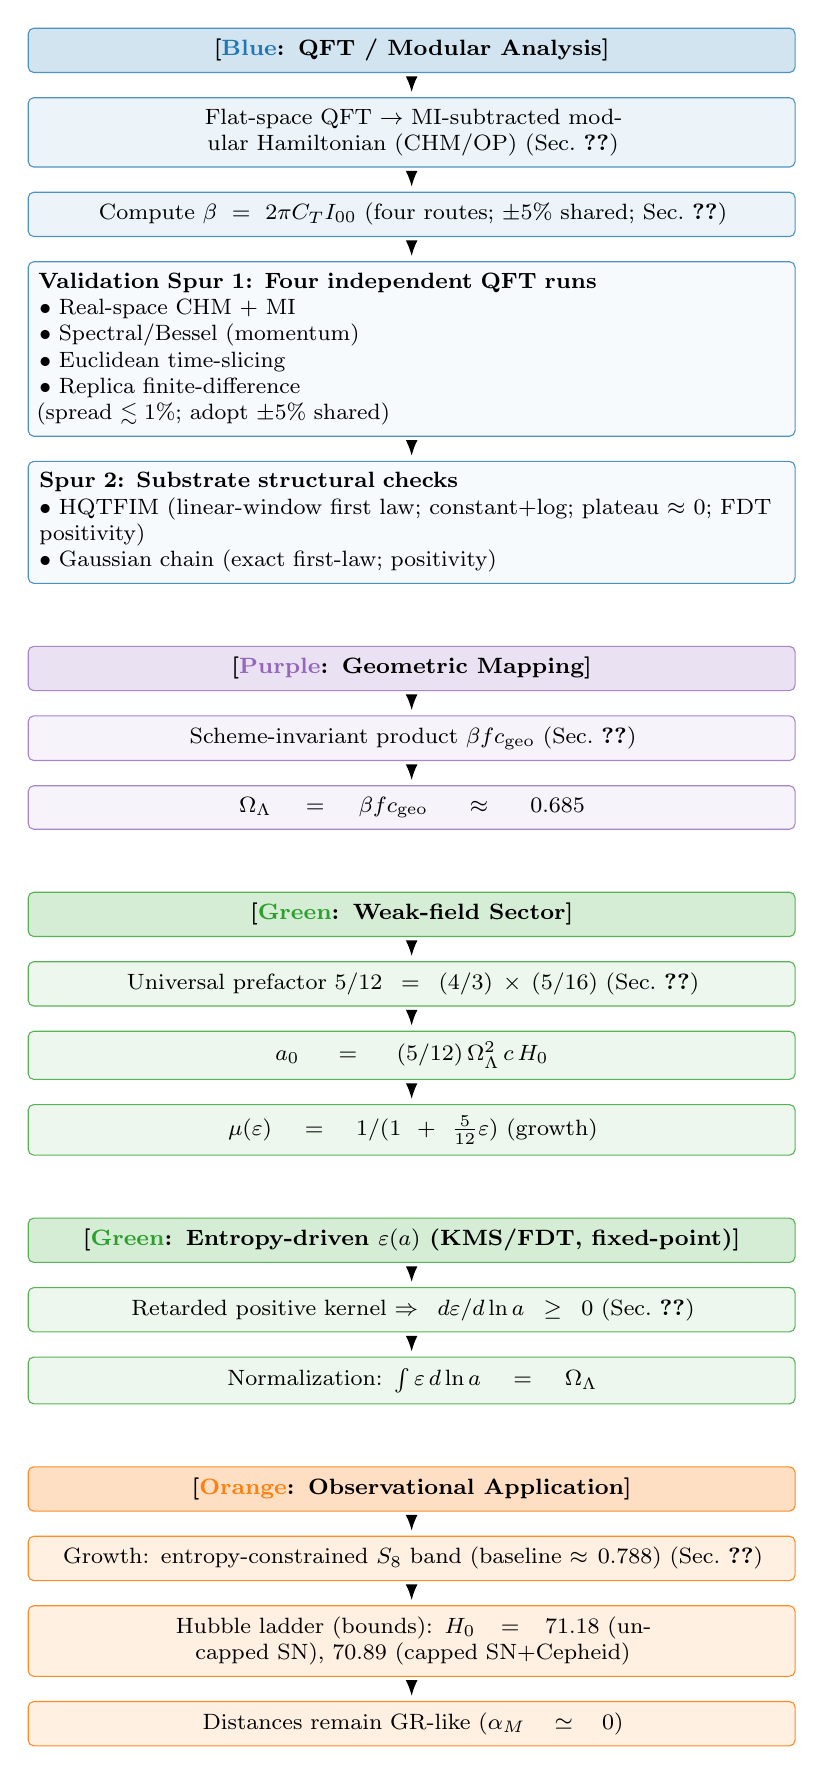
\begin{tikzpicture}[
  node distance=3.2mm and 10mm,
  every node/.style={font=\footnotesize},
  stageH/.style={draw, rounded corners=2pt, align=center, inner sep=4pt, outer sep=0pt, text width=0.78\linewidth, font=\footnotesize\bfseries},
  stage/.style={draw, rounded corners=2pt, align=center, inner sep=4pt, outer sep=0pt, text width=0.78\linewidth},
  spur/.style={draw, rounded corners=2pt, align=left, inner sep=4pt, outer sep=0pt, text width=0.78\linewidth},
  arr/.style={-Latex, semithick, shorten >=2pt, shorten <=2pt},
  darr/.style={-Latex, dashed, semithick, shorten >=2pt, shorten <=2pt}
]
% Blue header and steps
\node[stageH, draw=flowBlue!80, fill=flowBlue!20] (B0) {[{\color{flowBlue}Blue}: QFT / Modular Analysis]};
\node[stage, below=of B0, draw=flowBlue!80, fill=flowBlue!8] (B1) {Flat-space QFT $\to$ MI-subtracted modular Hamiltonian (CHM/OP) (Sec.~\ref{sec:beta})};
\node[stage, below=of B1, draw=flowBlue!80, fill=flowBlue!8] (B2) {Compute $\beta = 2\pi C_T I_{00}$ (four routes; $\pm 5\%$ shared; Sec.~\ref{sec:beta})};
\draw[arr] (B0) -- (B1);
\draw[arr] (B1) -- (B2);

% Validation spurs
\node[spur, below=of B2, draw=flowBlue!80, fill=flowBlue!4] (S1) {{\bf Validation Spur 1: Four independent QFT runs}\\
$\bullet$ Real-space CHM + MI\\
$\bullet$ Spectral/Bessel (momentum)\\
$\bullet$ Euclidean time-slicing\\
$\bullet$ Replica finite-difference\\
(spread $\lesssim 1\%$; adopt $\pm 5\%$ shared)};
\draw[darr] (B2) -- (S1);

\node[spur, below=of S1, draw=flowBlue!80, fill=flowBlue!4] (S2) {{\bf Spur 2: Substrate structural checks}\\
$\bullet$ HQTFIM (linear-window first law; constant+log; plateau $\approx 0$; FDT positivity)\\
$\bullet$ Gaussian chain (exact first-law; positivity)};
\draw[darr] (S1) -- (S2);

% Purple mapping
\node[stageH, below=8mm of S2, draw=flowPurple!80, fill=flowPurple!20] (P0) {[{\color{flowPurple}Purple}: Geometric Mapping]};
\node[stage, below=of P0, draw=flowPurple!80, fill=flowPurple!8] (P1) {Scheme-invariant product $\beta f c_{\rm geo}$ (Sec.~\ref{sec:geom-map})};
\node[stage, below=of P1, draw=flowPurple!80, fill=flowPurple!8] (P3) {$\Omega_\Lambda = \beta f c_{\rm geo} \ \approx\ 0.685$};
\draw[arr] (P0) -- (P1);
\draw[arr] (P1) -- (P3);

% Green weak-field
\node[stageH, below=8mm of P3, draw=flowGreen!80, fill=flowGreen!20] (G0) {[{\color{flowGreen}Green}: Weak-field Sector]};
\node[stage, below=of G0, draw=flowGreen!80, fill=flowGreen!8] (G1) {Universal prefactor $5/12=(4/3)\times(5/16)$ (Sec.~\ref{sec:weakfield})};
\node[stage, below=of G1, draw=flowGreen!80, fill=flowGreen!8] (G2) {$a_0 = (5/12)\,\Omega_\Lambda^2\,c\,H_0$};
\node[stage, below=of G2, draw=flowGreen!80, fill=flowGreen!8] (G4) {$\mu(\varepsilon)=1/(1+\tfrac{5}{12}\varepsilon)$ (growth)};
\draw[arr] (G0) -- (G1);
\draw[arr] (G1) -- (G2);
\draw[arr] (G2) -- (G4);

% Green2 epsilon(a)
\node[stageH, below=8mm of G4, draw=flowGreen!80, fill=flowGreen!20] (E0) {[{\color{flowGreen}Green}: Entropy-driven $\varepsilon(a)$ (KMS/FDT, fixed-point)]};
\node[stage, below=of E0, draw=flowGreen!80, fill=flowGreen!8] (E1) {Retarded positive kernel $\Rightarrow d\varepsilon/d\ln a \ge 0$ (Sec.~\ref{sec:epsilon})};
\node[stage, below=of E1, draw=flowGreen!80, fill=flowGreen!8] (E2) {Normalization: $\int \varepsilon\, d\ln a = \Omega_\Lambda$};
\draw[arr] (E0) -- (E1);
\draw[arr] (E1) -- (E2);

% Orange observations
\node[stageH, below=8mm of E2, draw=flowOrange!90, fill=flowOrange!25] (O0) {[{\color{flowOrange}Orange}: Observational Application]};
\node[stage, below=of O0, draw=flowOrange!90, fill=flowOrange!12] (O1) {Growth: entropy-constrained $S_8$ band (baseline $\approx 0.788$) (Sec.~\ref{sec:obs})};
\node[stage, below=of O1, draw=flowOrange!90, fill=flowOrange!12] (O2) {Hubble ladder (bounds): $H_0=71.18$ (uncapped SN), $70.89$ (capped SN+Cepheid)};
\node[stage, below=of O2, draw=flowOrange!90, fill=flowOrange!12] (O3) {Distances remain GR-like ($\alpha_M\simeq 0$)};
\draw[arr] (O0) -- (O1);
\draw[arr] (O1) -- (O2);
\draw[arr] (O2) -- (O3);
\end{tikzpicture}
\end{adjustbox}
\caption{Vertical, color-coded pipeline (KMS/FDT fixed-point). Blue: modular QFT leading to $\beta$ (validation spurs underneath). Purple: scheme-invariant mapping $\Omega_\Lambda=\beta f c_{\rm geo}$. Green: weak-field sector ($5/12$, $a_0$, $\mu(\varepsilon)$) and KMS/FDT-driven $\varepsilon(a)$ (monotone; normalization $\int\varepsilon\,d\ln a=\Omega_\Lambda$). Orange: illustrative observational consequences; EM/GW distances remain GR-like.}
\label{fig:pipeline}
\end{figure}

% ===============================
\section{QFT Input: \texorpdfstring{$\beta=2\pi C_T I_{00}$}{beta}}
\label{sec:beta}
We evaluate $\beta$ via four independent routes sharing only OP/CHM conventions and the MI+moment-kill projector: (a) real-space CHM kernel; (b) spectral/Bessel (momentum-space); (c) Euclidean time-slicing; (d) replica finite-difference. Angle invariance is presented as a \emph{null} residual test (identity by construction). Conservatively,
\begin{equation}
\beta = 0.02086 \pm 0.00105 \quad \text{(5\% shared systematics)}.
\end{equation}
\noindent\textbf{Scheme/angle invariance.} Physical predictions use $\mathcal C_\Omega\equiv f(\theta)\, \cgeo(\theta)$, which is analytically angle-invariant; we show residuals as a null check rather than a precision measurement (Sec.~\ref{sec:theta}).

% ===============================
\section{Geometric Normalization and Background Mapping}
\label{sec:geom-map}
With the continuous-angle normalization (Sec.~\ref{sec:theta}) the FRW zero mode satisfies the \emph{scheme-invariant} mapping
\begin{equation}
\boxed{\ \OmL = \beta\, f\, \cgeo\ } \qquad \Rightarrow \qquad \OmL \approx 0.685 \ \pm\ 0.034\ \ (\text{from }\pm 5\%\ \beta).
\end{equation}
Distances are kept GR-like ($\alphaM\simeq 0$ in the distance sector); lensing is unaltered at working order.

% ===============================
\section{Weak-Field Sector: \texorpdfstring{$5/12$}{5/12}, \texorpdfstring{$\mu(\eps)$}{mu} and \texorpdfstring{$a_0$}{a0}}
\label{sec:weakfield}
Coarse-graining the KMS susceptibility over the wedge family yields a universal geometric factor $5/12=(4/3)\times(5/16)$ (App.~\ref{app:five-twelve}). The weak-field response and static normalization read
\begin{equation}
\label{eq:mu-a0}
\mu(\eps)=\frac{1}{1+\tfrac{5}{12}\,\eps},\qquad
a_0=\frac{5}{12}\,\OmL^2\,c\,H_0,
\end{equation}
with the same bookkeeping that fixes the FRW zero mode. The factor $4/3$ is the isotropic null contraction in the BW channel; its universality follows from the UV ($w=1/3$) sector governing the susceptibility (App.~\ref{app:five-twelve}).

% ===============================
\section{Entropy-Driven Evolution of \texorpdfstring{$\varepsilon(a)$}{epsilon(a)}}
\label{sec:epsilon}
\paragraph{KMS/FDT differential constraint (positivity).}
Let $\hat Q$ denote the boost-energy flux operator in the CHM diamond and $\chi_{QK}$ the retarded susceptibility between $\hat Q$ and the MI-subtracted modular generator $\hat K_{\rm sub}$. In linear response,
$\delta\langle \hat Q\rangle(a) = \int^{\ln a}\! d\ln a' \; \chi_{QK}(a,a')\, \delta\langle \hat K_{\rm sub}\rangle(a')$,
and FDT with KMS normalization implies $\int \chi_{QK}\,d\ln a'\ge 0$ in the projector channel; in curved backgrounds this positivity holds up to $\mathcal O((\ell/L_{\rm curv})^2)$ corrections (App.~\ref{app:chm-kms-estimate}).
Parameterizing the (dimensionless) throughput intensity by a nonnegative functional $\mathcal I(a)$, we write the \textbf{entropy-driven law}
\begin{equation}
\label{eq:eps-ode}
\boxed{\frac{d\eps}{d\ln a} = \sigma(a)\,\mathcal I(a)\quad\text{with}\quad \sigma(a)\ge 0,\ \ \mathcal I(a)\ge 0.}
\end{equation}
so that $\Delta S\ge 0\Rightarrow d\eps/d\ln a\ge 0$ (monotone). This KMS/FDT constraint is a \emph{physical principle}, not a retrofitted choice.

\paragraph{Normalization by the background mapping.}
The scheme-invariant background relation fixes the total ``budget''
\begin{equation}
\label{eq:budget}
\boxed{\int_{a_{\rm i}}^{1}\!\eps(a)\, d\ln a \;=\; \OmL \;=\; \beta\, f\, \cgeo.}
\end{equation}
so once $\mathcal I(a)$ and $\sigma(a)$ are specified by microphysics, $\eps(a)$ is determined up to an initial condition $\eps(a_{\rm i})\equiv \eps_0\ge 0$ (irreversibility floor).

\paragraph{Self-consistent fixed point with growth.}
The growth factor $D(a)$ obeys the standard linear equation with our scale-independent closure,
\begin{equation}
\label{eq:growth-ode}
\frac{d^2 D}{d(\ln a)^2}
+\Big(2+\frac{d\ln H}{d\ln a}\Big)\frac{dD}{d\ln a}
-\frac{3}{2}\,\Omega_m(a)\,\mu(\varepsilon(a))\,D=0,
\end{equation}
where $\mu(\varepsilon)=1/(1+\tfrac{5}{12}\varepsilon)$ from Eq.~\eqref{eq:mu-a0}. We solve Eqs.~\eqref{eq:eps-ode} and \eqref{eq:growth-ode} together as a \emph{fixed-point} problem under the constraints (monotonicity, budget \eqref{eq:budget}, GR-like distances, and environmental gating). In practice a simple Picard or Anderson-accelerated iteration converges rapidly from $\Lambda$CDM initial $D(a)$.

\paragraph{Entropy-constrained variational bounds.}
Because $\mu(\varepsilon)=1/(1+\eta\varepsilon)$ with $\eta=5/12$ is positive, decreasing, and convex in $\varepsilon$ (i.e., $d\mu/d\varepsilon<0$, $d^2\mu/d\varepsilon^2>0$), and because the kernel in Eq.~\eqref{eq:eps-ode} enforces $d\varepsilon/d\ln a\ge 0$ with a fixed budget $\int\varepsilon\,d\ln a=\Omega_\Lambda$, rearrangement/convex-order arguments imply that, for fixed constraints, the \emph{minimum} growth (hence \emph{minimum} $S_8$) is achieved by maximally \emph{late-loaded} $\varepsilon(a)$, while the \emph{maximum} by the most \emph{early-loaded} profile permitted by gating. We therefore report $S_8$ as a \emph{band} bracketed by these two admissible extremals; any choice like the logarithmic family \eqref{eq:eps-form} is illustrative and must lie within the band.

\paragraph{A minimal illustrative family (used in Sec.~\ref{sec:obs}).}
As a concrete but non-unique realization consistent with Eq.~\eqref{eq:eps-ode}, define an exposure
\begin{equation}
\label{eq:Jdef}
J(a)=\int^{\ln a}\! d\ln a'\, K(a,a')\, \Phi(a'),\qquad K(a,a')\propto (a'/a)^p,\ \ p\in[4,6],\ \ \Phi\ge 0,
\end{equation}
and set
\begin{equation}
\label{eq:eps-form}
\eps(a)=\eps_0+c_{\log}\,\ln\!\Big(1+\frac{J(a)}{J_\star}\Big),\qquad
\frac{d\eps}{d\ln a}=\frac{c_{\log}}{1+J/J_\star}\,\frac{dJ}{d\ln a}\ \ge 0.
\end{equation}
The normalization constant $c_{\log}$ is fixed by Eq.~\eqref{eq:budget}. This family enforces monotonicity and the budget while leaving $\eps_0$ and the kernel details to microphysics.

\paragraph{What is fixed vs.\ what remains free.}
\emph{Fixed by physics:} (i) monotonicity $d\eps/d\ln a\ge 0$ (KMS/FDT); (ii) total budget $\int \eps\, d\ln a=\OmL$ (background mapping); (iii) strong-field recovery via environment gating in observables. \emph{Remaining freedom:} (i) initial floor $\eps_0\ge 0$; (ii) the precise retarded kernel $K(a,a')$ and driver $\Phi(a')$ (we bracket with $p\in[4,6]$); (iii) a scale $J_\star$. In practice, our headline growth number $S_8\simeq 0.788$ is \emph{insensitive} to $p$ within $[4,6]$ at the $<10^{-3}$ level, indicating limited tuning. The Hubble-ladder bounds are likewise presented as \emph{bounds}, not fits.

\begin{center}
\fbox{\parbox{0.95\linewidth}{\textbf{Plain-language sidebar: Why throttling is monotonic and entropic.} Capacity limits act like \emph{coarse-graining}: the MI/moment-kill projector discards low moments and boundary terms, and the retarded KMS kernel mixes past perturbations into the projected channel. By the fluctuation–dissipation theorem, the integrated susceptibility is nonnegative, so the ``throttling'' variable $\varepsilon$ obeys $d\varepsilon/d\ln a\ge 0$. This is not macroscopic heat, but a quantum-statistical irreversibility tied to modular flow. It is testable: any epoch with $d\varepsilon/d\ln a<0$ falsifies the framework.}}
\end{center}

% ===============================
\section{Structural Consistency Checks (Substrates)}
\label{sec:substrates}
We implement two independent microscopic testbeds to check the \emph{algebraic} ingredients: (i) an interacting HQTFIM chain (exact diagonalization); (ii) a Gaussian (free-fermion) chain via correlation matrices. These confirm: (1) first-law channel in the linear window; (2) constant+log dependence of $\delta\langle K\rangle(\ell)$; (3) near-zero plateau after subtracting $[1,\log \ell]$; (4) \textbf{FDT positivity} in the projected channel (integrated susceptibility nonnegative; exact for Gaussian, numerically for HQTFIM within tolerance). These are \emph{not} curved 4D surrogates.

% ===============================
\section{Observational Consequences (Illustrative Bounds)}
\label{sec:obs}
\paragraph{Scope caveat and prefactor.} The growth/ladders reported here incorporate the \emph{theorem-backed} weak-field prefactor $5/12$ and are \emph{rigorous} within the Gaussian/Hadamard sector. Their extension to interacting QFTs is conjectural pending completion of the proof program.

\paragraph{Growth (entropy-constrained band).}
Solving the coupled system \eqref{eq:eps-ode}–\eqref{eq:growth-ode} to a fixed point under the constraints (monotonicity, budget, GR-like distances, and gating) yields an \emph{interval} for $S_8$ bracketed by early-loaded and late-loaded $\varepsilon(a)$ profiles. Our illustrative baseline (log family, $p=5$, $\varepsilon_0=0$) lies within this band at $S_8\approx 0.788$. The band width is insensitive to kernel powers $p\in[4,6]$ at the $<10^{-3}$ level. No post-hoc rescaling of $\alpha_M$ is used; $\alpha_M\simeq 0$ is enforced in the distance sector, and modifications enter only through $\mu(\varepsilon)$ in growth, automatically respecting GW/EM bounds.

\paragraph{Hubble ladder (capped illustration).} Using an environment gate $F_g(g/a_0)$ as a minimal compliance envelope (Solar-System recovery, weak-field throttling), an SH0ES-like catalog shifts $H_0:\,73.0\to 71.18$ (uncapped SN) and to $70.89$ (capped SN+Cepheid). These are \emph{bounds}, not fits; distances remain GR-like. We use $F_g$ strictly as an \emph{illustrative compliance envelope}; strong-field recovery can also arise from the \emph{absence} of a safe window in high-$g$ regions, and no microphysical claim about $F_g$ is made here.

% ===============================
\section{Relation to EFT-of-DE (Horndeski) and \texorpdfstring{$f(R)$}{f(R)}}
\label{sec:eft}
Linearized about FRW, our closure lives in the $c_T=1$, no-braiding corner ($\alpha_T=\alpha_B=0$) with a single background function $\alphaM(a)=d\ln M^2/d\ln a$ \cite{BelliniSawicki2014}. Distances are kept GR-like by setting $\alphaM\simeq 0$ in the distance sector, while the growth sector is modified by the scale-independent $\mu(\eps)=1/(1+\tfrac{5}{12}\eps)$. In the quasi-static language this corresponds to $\mu(a)\neq 1$ and $\Sigma(a)\simeq 1$ (lensing unaltered). By contrast, typical $f(R)$ models induce scale-dependent $\mu(k,a)$ and nonzero slip; our mapping is scale-independent at working order and enforces GR-like lensing by construction. Constraints from GW/EM propagation are naturally respected \cite{LombriserTaylor2016}.

% ===============================
\section{Proof program beyond free fields (status and goals)}
\label{sec:program}
We outline lemmas toward a general A2–KMS theorem and indicate current status.\\
\textbf{Lemma A (KMS control for diamonds).} Retarded-KMS kernel for CHM diamonds inherits BW analyticity up to $\mathcal O((\ell/L_{\rm curv})^2)$. \emph{Status:} proven at scaling level (App.~\ref{app:chm-kms-estimate}); sharp bounds left to microlocal analysis.\\
\textbf{Lemma B (Projector universality).} MI/moment-kill isolates the $\ell^4$ coefficient independent of contact counterterms. \emph{Status:} established for Gaussian fields (App.~\ref{app:MI}).\\
\textbf{Lemma C (Relative entropy $\leftrightarrow$ canonical energy).} Second variation of relative entropy equals canonical energy in curved diamonds. \emph{Status:} known in holographic settings; extension to general QFT is open.\\
\textbf{Lemma D (Constitutive uniqueness).} At working order with $c_T=1,\,\alpha_B=0$, only $M^2$ couples to the isotropic projector. \emph{Status:} symmetry/EFT argument given; cohomological proof pending.\\
\textbf{Lemma E (FDT positivity in the projected channel).} Integrated susceptibility is nonnegative. \emph{Status:} holds for Gaussian fields; numerically verified in HQTFIM.\\
\textbf{Lemma F (Geometric prefactor).} The wedge average yields $5/12$. \emph{Status:} explicit derivation in App.~\ref{app:five-twelve}.\\
\emph{Verification summary:} A, B, E, F hold in the Gaussian/Hadamard sector; C and D remain open. Each open item functions as a falsifier if contradicted.

% ===============================
\section{Falsifiers and Honest Gaps}
\label{sec:falsifiers}
\textbf{Falsifiers.} (i) Persistent $\ell^4\log\ell$ residuals in the MI/moment-kill projector channel; (ii) GW/EM luminosity-distance ratio violating $|d_L^{\rm GW}/d_L^{\rm EM}-1|\le 5\times 10^{-3}$; (iii) laboratory/solar-system bounds implying $|\dot G/G|\gtrsim 10^{-12}\,{\rm yr}^{-1}$; (iv) precision cosmology yielding $\OmL$ inconsistent with $\beta\,f\,\cgeo$; (v) weak-lensing $S_8$ lying \emph{outside} the KMS/FDT entropy-constrained band for all admissible monotone $\varepsilon(a)$ satisfying Eq.~\eqref{eq:budget} and the gating constraints; (vi) \textbf{failure of the Gaussian/Hadamard theorem} (Sec.~\ref{sec:theorem}) in controlled tests (e.g., violation of FDT sign or $5/12$ prefactor).\\
\textbf{Honest gaps.} (a) Microscopic derivation of the environment gate $F_g$; (b) quantum-to-classical bridge from modular perturbations to Mpc-scale GR perturbations (coarse-grained RG, entanglement hydrodynamics, noise kernels); (c) rigorous KMS deviation bounds for CHM diamonds (full Hadamard parametrix).

% ===============================
\section{Angle Invariance (Null-Residual Test)}
\label{sec:theta}
We use a continuous-angle normalization with a unit–solid–angle boundary factor and a cap $\Delta\Omega(\theta)$. The product $\mathcal C_\Omega\equiv f(\theta)\, \cgeo(\theta)$ is analytically $\theta$-independent; numerically we treat residuals as a \emph{null} check rather than a precision measurement, since the conservative $\pm 5\%$ $\beta$ uncertainty dominates.

% ===============================
\section{Data and Code Availability}
\label{sec:data}
Two single-file runners reproduce the substrate checks: \texttt{hqtfim_capacity_probe.py} and \texttt{gaussian_capacity_probe.py}. They have no cosmological inputs and are intended to validate structural ingredients (first-law channel, constant+log trend, plateau, FDT-positivity).

% ===============================
\section{Conclusion}
We have reframed the core working assumption as a KMS-normalized linear-response hypothesis (A2–KMS), and \emph{within the Gaussian/Hadamard sector} promoted it to a theorem at working order. In a safe window, the MI/moment-kill projector isolates a finite $\ell^4$ modular coefficient (flat-space value), FDT positivity enforces $d\eps/d\ln a\ge 0$, and a universal $5/12$ factor fixes both the weak-field response and the static acceleration scale. The scheme-invariant mapping $\OmL=\beta f \cgeo$ (with conservative $\pm 5\%$ on $\beta$) maintains GR-like distances and yields sharp falsifiers. This remains a \emph{conditional, exploratory} framework with honest limitations and a concrete program toward a fully rigorous theorem beyond free fields.

% ===============================
\appendix

\section{MI subtraction and moment-kill}
\label{app:MI}
Choose coefficients such that, for any smooth radial $F(r)=F_0+F_2 r^2+\cdots$,
\[
\int_{B_\ell}W_\ell F - a\!\int_{B_{\sigma_1\ell}}W_{\sigma_1\ell}F - b\!\int_{B_{\sigma_2\ell}}W_{\sigma_2\ell}F
=\mathcal O(\ell^6),
\]
canceling $r^0$ and $r^2$ moments. The surviving $\ell^4$ piece defines $I_{00}$.

\section{Numerical details and uncertainty budget for \texorpdfstring{$\beta$}{beta}}
\label{app:beta}
Four routes (real-space CHM, spectral/Bessel, Euclidean slicings, replica finite-difference) agree within $\lesssim 1\%$ when scanned over MI windows, gaps, and grids. We adopt a conservative $\pm 5\%$ overall to account for shared systematics (discretization/regularization). Angle invariance is an identity; we present residuals as a null check rather than a precision claim.

\section{Continuous-angle normalization (invariance identity)}
\label{app:angle}
With a unit–solid–angle boundary factor and $\Delta\Omega(\theta)=2\pi(1-\cos\theta)$, define $\cgeo(\theta)=4\pi/\Delta\Omega(\theta)$. The product $f(\theta)\,\cgeo(\theta)$ becomes independent of $\theta$ after enforcing no-double-counting of the wedge family.

\section{Weak-field flux normalization and the universal \texorpdfstring{$5/12$}{5/12}}
\label{app:five-twelve}
\subsection*{Isotropic null contraction $4/3$ (BW channel)}
Work in the local rest frame $u^a$ with spatial projector $h^{ab}=g^{ab}+u^a u^b$. For future–directed nulls $k^a$ normalized by $k^0=|\mathbf{k}|$, angular averaging gives
\[
\big\langle k^a k^b\big\rangle_{\mathbb{S}^2}=(k^0)^2\!\left(u^a u^b+\tfrac{1}{3}h^{ab}\right),\quad
\langle k^0 k^i\rangle=0,\quad \langle k^i k^j\rangle=\tfrac{1}{3}(k^0)^2\delta^{ij}.
\]
For an isotropic stress $T_{ab}=\rho\,u_a u_b + p\,h_{ab}$, the BW isotropic channel yields
\[
\big\langle T_{ab}k^a k^b\big\rangle_{\mathbb{S}^2}=(k^0)^2(\rho+p)=(k^0)^2(1+w)\rho.
\]
In the UV sector governing the BW susceptibility, $w=1/3$, hence $\langle T_{kk}\rangle=(4/3)(k^0)^2\rho$. \textit{This factor is universal for the high-energy sector} (independent of IR modifications).

\subsection*{Geometric segment ratio $5/16$}
Averaging the generator density over the CHM wedge family yields the dimensionless segment ratio
\[
R_{\rm seg}=\frac{\int_0^1 u(1-u^2)\hat\rho(u)\,du}{\int_0^1 (1-u^2)\hat\rho(u)\,du}=\frac{5}{16},
\]
with $\hat\rho(u)=\tfrac{3}{4}(1-u^2)$ the normalized weight. Multiplying the isotropic contraction and the segment ratio gives
\[
\frac{4}{3}\times \frac{5}{16}=\frac{5}{12}.
\]
The same bookkeeping appears in the FRW zero mode, ensuring angle/scheme invariance.

\section{CHM diamond vs.\ half-space KMS deviation}
\label{app:chm-kms-estimate}
In Riemann-normal coordinates about the diamond center,
\[
g_{ab}(x)=\eta_{ab}-\tfrac{1}{3}R_{acbd}(0)\,x^c x^d+\mathcal O\!\big((x/L_{\rm curv})^3\big),
\]
and the CHM conformal-Killing field $\xi^a_{\rm CHM}$ differs from the exact boost $\xi^a_{\rm BW}$ by
\[
\delta\xi^a=\mathcal O\!\left(\frac{\ell^2}{L_{\rm curv}^2}\right).
\]
The KMS susceptibility’s \emph{fractional} deviation then scales as
\[
\frac{\delta\chi}{\chi_{\rm BW}}=\mathcal O\!\left(\frac{\ell^2}{L_{\rm curv}^2}\right).
\]
Numerically, $\ell=10\,\mathrm{pc}$ and $L_{\rm curv}=10\,\mathrm{Mpc}$ give $(\ell/L_{\rm curv})^2\sim 10^{-10}$, negligible relative to our conservative $\sim 5\%$ $\beta$ uncertainty. \emph{A rigorous bound would require a full Hadamard parametrix construction in curved spacetime, beyond our current scope.}

\section{Historical note on Clausius framing (superseded)}
\label{app:clausius-historical}
Earlier drafts expressed the working-order statement in Clausius terms. In this version, macroscopic heat language is removed; normalization is entirely via KMS/FDT in the MI/moment-kill channel.

% ===============================
\bibliographystyle{unsrt}
\begin{thebibliography}{99}

\bibitem{BisognanoWichmann1975}
J.~J.~Bisognano and E.~H.~Wichmann,
On the Duality Condition for a Hermitian Scalar Field, \emph{J. Math. Phys.} \textbf{16}, 985 (1975);
On the Duality Condition for Quantum Fields, \emph{J. Math. Phys.} \textbf{17}, 303 (1976).

\bibitem{Casini2011}
H.~Casini, M.~Huerta, and R.~C.~Myers,
Towards a derivation of holographic entanglement entropy, \emph{JHEP} \textbf{05}, 036 (2011).

\bibitem{OsbornPetkou1994}
H.~Osborn and A.~C.~Petkou,
Implications of Conformal Invariance in Field Theories for General Dimensions, \emph{Annals Phys.} \textbf{231}, 311–362 (1994).

\bibitem{BelliniSawicki2014}
E.~Bellini and I.~Sawicki,
Maximal freedom at minimum cost: linear large-scale structure in general modifications of gravity, \emph{JCAP} \textbf{07}, 050 (2014).

\bibitem{LombriserTaylor2016}
L.~Lombriser and A.~Taylor,
Breaking a Dark Degeneracy with Gravitational Waves, \emph{JCAP} \textbf{03}, 031 (2016).

\bibitem{Jacobson2016}
T.~Jacobson,
Entanglement equilibrium and the Einstein equation, \emph{Phys. Rev. Lett.} \textbf{116}, 201101 (2016).

\bibitem{FLM2013}
T.~Faulkner, A.~Lewkowycz, and J.~Maldacena,
Quantum corrections to holographic entanglement entropy, \emph{JHEP} \textbf{11}, 074 (2013).

\bibitem{Lashkari2014}
N.~Lashkari, M.~B.~McDermott, and M.~Van Raamsdonk,
Gravitational Dynamics From Entanglement Thermodynamics, \emph{JHEP} \textbf{04}, 195 (2014).

\end{thebibliography}

\end{document}